\subsection{Single Shot MultiBox Detector}

Zwar liefern die oben genannten Objektdetektoren akkurate Ergebnisse, allerdings sind sie als zu rechenintensiv und langsam einzuordnen, als dass sie für Echtzeit Applikationen eingesetzt werden könnten. Der \textit{Single Shot MultiBox Detector} (SSD) unterschiedet sich von den vorhergegangenen Modellen dahingehend, dass er bewusst auf den Schritt der Generierung von Bounding Box Vorschlägen und des \textit{Poolings} verzichtet, um wesentlich schneller ablaufen zu können als andere Objektdetektoren. Die Präzision der Klassifikationen bleibt hierbei erhalten, selbst Bilder niedriger Auflösung können weiterhin verarbeitet werden. Dem \textit{SSD} genügt also ein einziges tiefes neuronales Netz zum Lokalisieren und Klassifizieren von Objekten. Wie der \textit{SSD} aufgebaut ist und welche Ansätze er verfolgt, soll in diesem Unterkapitel erläutert werden. \cite[S. 1f.]{ssd.20161229}. 

\begin{figure}[ht]
	\begin{center}
		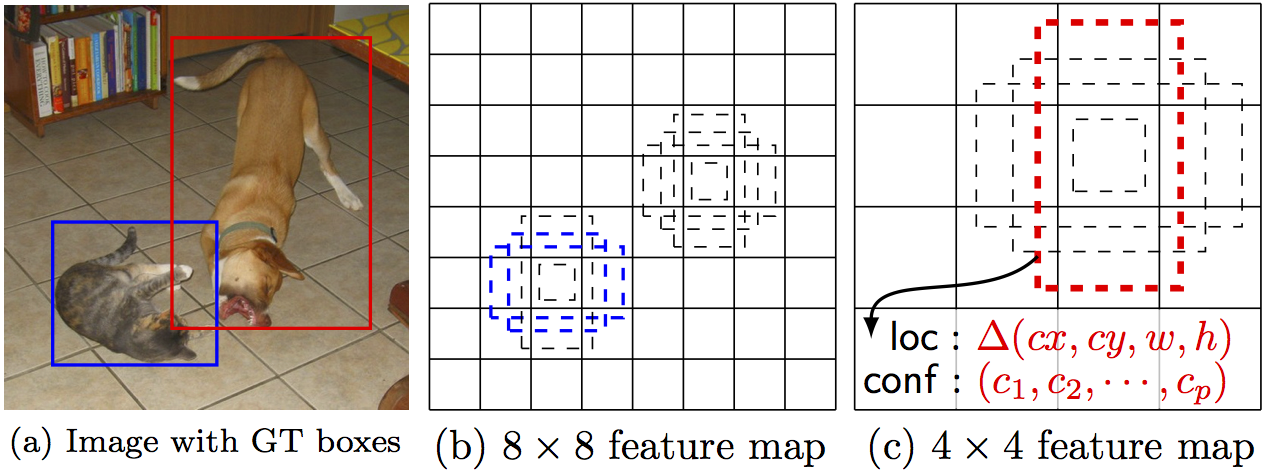
\includegraphics[width=15cm]{Bilder/ssd_framework.png} 
		\caption[SSD Grundprinzip]{SSD Grundprinzip \cite[S. 3]{ssd.20161229}}
		\label{framework}
	\end{center}
\end{figure}

Die Architektur des \textit{SSD} zielt zunächst darauf ab, ein Bild in mehrere unterschiedliche Gitterstrukturen zu unterteilen, die sich nach ihrer Skalierung unterscheiden. Dadurch ist es möglich Objekte unterschiedlicher Größe zu erkennen. Jede Lokation im Gitter besitzt eine gleiche Anzahl an festen, vordefinierten Bounding Boxen, die unterschiedliche Seitenverhältnisse aufweisen (siehe Abbildung \ref{framework}). So wird sichergestellt, dass sowohl horizontal als auch vertikal ausgeprägte Objekte in der selben Lokation gleichzeitig erkannt werden können (siehe Abbildung \ref{boundingboxes}). \cite[S. 3]{ssd.20161229}

\begin{figure}[ht]
	\begin{center}
		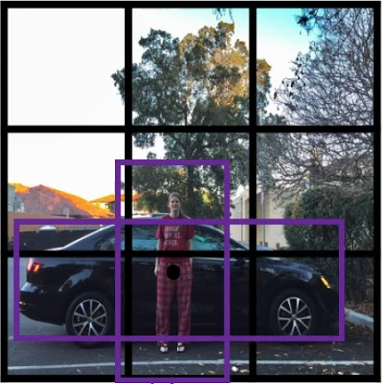
\includegraphics[width=7cm]{Bilder/bounding_boxes.png} 
		\caption[Bounding Boxes]{Bounding Boxes \cite{AndrewNg.2019}}
		\label{boundingboxes}
	\end{center}
\end{figure}

Für jede dieser Bounding Boxen bestimmt der \textit{SSD} Wahrscheinlichkeiten für Klassenzugehörigkeiten als auch Verschiebungen der vordefinierten Bounding Box zur wahren Bounding Box des Objekts für jede Klasse. Dies wird mit kleinen Faltungsfiltern erreicht, die in den hinteren Schichten des Netzwerks eingesetzt werden. \cite[S. 3]{ssd.20161229}

Die Kostenfunktion ist durch die gewichtete Summe des Lokalisationsverlustes und des Klassifikationsverlustes bestimmt. Während der Klassifikationverlust durch eine \textit{Softmax} Funktion bestimmt werden kann, wird der Lokalisationsverlust über die \textit{Smooth L1} Funktion bestimmt (siehe Formel \ref{smooth}). \cite[S. 3]{ssd.20161229}

\begin{equation}\label{smooth}
\begin{split}
L_{loc}(t^u,v) = \sum\limits_{x \in {x,y,w,h}}^{n} smooth_{L1}(t^u_i - v_i) \\
smooth_{L1}(t^u_i - v_i) = \begin{cases}
							0.5x^2      & \text{wenn } |x| < 1\\
							|x| - 0.5   & \text{sonst}
						   \end{cases}
\end{split}
\end{equation}
\equations{Die Smooth L1 Funktion}

\begin{figure}[ht]
	\begin{center}
		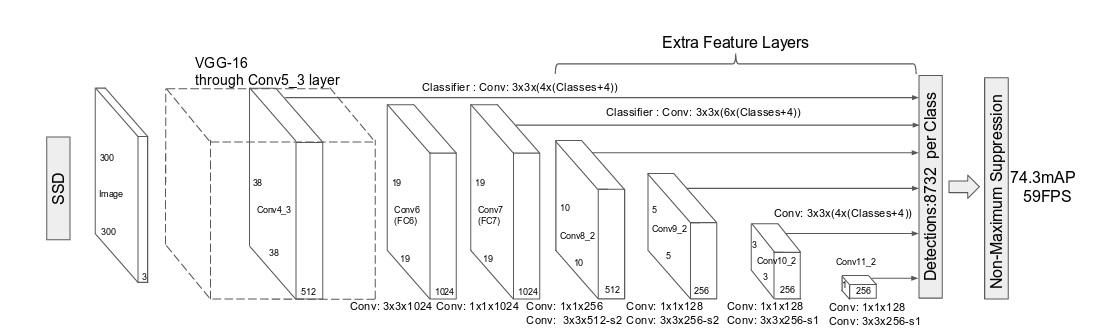
\includegraphics[width=15cm]{Bilder/ssd_architecture.png} 
		\caption[SSD Architektur]{SSD Architektur \cite[S. 4]{ssd.20161229}}
		\label{architecture}
	\end{center}
\end{figure}

Der \textit{SSD} benutzt ein \textit{VGG-16} Basis Netzwerk, um Klassifikationen zu ermöglichen. \textit{VGG-16} ist ein auf dem Datensatz von \textit{ImageNet} basierendes neuronales Netz, dass bis zu 1000 unterschiedliche Kategorien klassifizieren kann \cite{MathWorks.2019b}. Unabhängig vom Basisnetzwerk werden Convolutional Layer als Hilfsstrukturen zur Objektdetektion eingesetzt. Diese teilen das Bild in die gitterförmigen Lokationen ein, wobei die Gittergröße mit fortschreitenden Convolutional Layern zunimmt. Jeder Convolutional Layer kann eine feste Anzahl an Detektionen bestimmen. Eine Detektion wird durch eine Klassenangabe und die Lage einer vorhergesagten Bounding Box bestimmt. Eine Bounding Box wird durch einen Eckpunkt $P(x,y)$ und eine Höhe und Breite bestimmt. Bei $c$ Klassen hat der Ausgangsvektor demnach die Größe $c+4$. Die Koordinaten werden dabei relativ zur Lokation und zur standardmäßig festgelegten Bounding Box angegeben. Bei $m \cdot n$ Lokationen und $k$ verschiedenen Standardboxen pro Lokation ergeben sich also $m \cdot n \cdot k \cdot (c+4)$ verschiedene Werte für eine Feature Map. Die Merkmalsextraktion zur Klassifikation wird durch Faltung mit $3x3$ Filtern erreicht. \cite[S. 3]{ssd.20161229} 

Dieser Vorgang wird für alle Feature Maps für alle Convolutional Layer durchgeführt. Die daraus folgende Menge an Detektionen wird durch ein \textit{Non Maximum Suppression Layer} in ihrer Größe reduziert. Als Maß zur Filterung wird die sogenannte \textit{Intersection over Union} (IoU) der detektierten Box zur wahren Box verwendet (siehe Abbildung \ref{iou}). \cite[S. 3]{ssd.20161229} 

\begin{figure}[ht]
	\begin{center}
		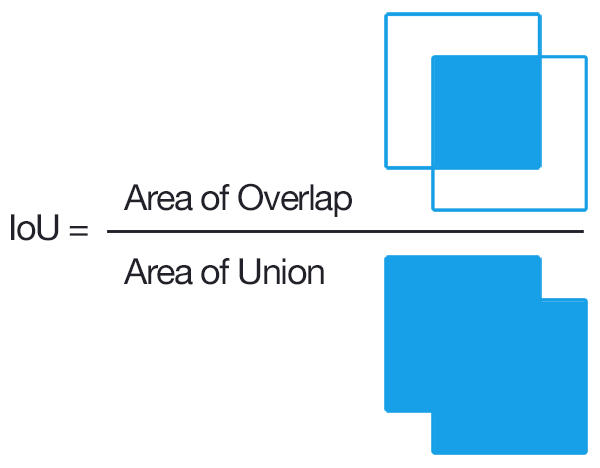
\includegraphics[width=8cm]{Bilder/iou_equation.png} 
		\caption[Intersection over Union]{Intersection over Union \cite{AdrianRosebrock.20161107}}
		\label{iou}
	\end{center}
\end{figure}

- gut/einfach zu trainieren, zu integrieren, zu interferieren
- 74.3 mAP (VOC 2007), 59 FPS Titan X (300)
	- Faster R-CNN: 7FPS, 73.2 maP
	- YOLO: 45 FPS, 63.4 maP
- 76.9 mAP (512)
